\documentclass[
  a4paper,
  12pt,
  dvipdfmx
]{article}
\usepackage{titling}
\usepackage{amsmath,amssymb}
\usepackage{amsthm} %定理環境
\usepackage{bm}
\usepackage{url}
\usepackage[dvipdfmx]{graphicx, color}
\usepackage{ascmac}
\usepackage{enumerate} %箇条書き
\usepackage{enumitem}
\usepackage{mathtools}
\usepackage{amsfonts}
\usepackage{latexsym}
% \usepackage[all]{xy}
% \usepackage{ulem} %波線
\usepackage[normalem]{ulem}
% %\usepackage{eclbkbox}%四角枠 
\usepackage{tocloft}%体裁を整える
\usepackage{titlesec}%見出しの設定
\usepackage{float}%図の位置
\usepackage{mathrsfs}%花文字
\usepackage{tikz}
\usepackage[dvipdfmx]{hyperref}
\usepackage{pxjahyper} % (u)pLaTeXのときのみかく
\usepackage{docmute} %分割に必要 
\usepackage{tikz-cd} %可換図式
% \usepackage[margin=30truemm]{geometry}
% \usepackage{authblk}
\usetikzlibrary{arrows.meta}
\usetikzlibrary{patterns}
\usetikzlibrary{spath3}
\usetikzlibrary{knots}
\usetikzlibrary{hobby}
\usetikzlibrary{external}

%自分用のコマンド
\providecommand{\cprime}{\hbox{$'$}} %bibtex用
\newcounter{questionCounter}% 新しいカウンターを定義
\newcommand{\Qbox}{\stepcounter{questionCounter}\fbox{\thequestionCounter}}
\newcommand{\RR}{\mathbb{R}}
\newcommand{\CC}{\mathbb{C}}
\newcommand{\engname}[1]{(\textit{#1})}
\newcommand{\te}{\textrm{there exists\ }}
\newcommand{\st}{\ \textrm{such that}\ }
\newcommand{\mcal}[1]{\mathcal{#1}}
\newcommand{\fall}{\textrm{for all}\ }
\newcommand{\suml}[2]{\sum\limits_{#1}^{#2}}
\newcommand{\simpangle}[1]{\langle#1\rangle}
\newcommand{\ZZ}{\mathbb{Z}}
\newcommand{\NN}{\mathbb{N}}
\newcommand{\QQ}{\mathbb{Q}}
\newcommand{\ca}{\mathcal{A}}
\newcommand{\ck}{\mathcal{K}}
% 卒論
\setlength{\topmargin}{0truecm}
\newcommand{\TITLE}%
{Homomorphic Expansions for Knotted Trivalent Graphs}
\newcommand{\STNO}%
{2264246}
\newcommand{\NAME}%
{宮路 宙澄}%氏名
\newcommand{\ADVR}%
{野崎 雄太 准教授}
\newcommand{\DATE}%
{(2026年1月30日)}
\DeclareMathOperator{\Ker}{Ker}
\DeclareMathOperator{\rank}{rank}
\DeclareMathOperator{\gr}{gr} %graded
\DeclareMathOperator{\id}{id} %id
\DeclareMathOperator{\proj}{proj}

\let\Re\relax%実部虚部の更新
\DeclareMathOperator{\Re}{Re}
\let\Im\relax
\DeclareMathOperator{\Im}{Im}

\title{
  \centerline{\mbox{卒論(タイトル未定)}}
  % Jones 多項式と Vassiliev 不変量の導入と関係性\\
  \large 元論文: Homomorphic expansions for knotted trivalent graphs
}
\author{宮路 宙澄}
\date{\today}
\hypersetup{
  colorlinks=false,
  pdfborder={0 0 1},
  linkbordercolor={red},
}

\renewcommand{\theenumi}{\roman{enumi}}
\renewcommand{\labelenumi}{(\theenumi)}
\renewcommand{\theenumii}{\theenumi-\alph{enumii}}
\renewcommand{\labelenumii}{(\theenumii)}
\renewcommand{\theenumiii}{\theenumii-\roman{enumiii}}
\renewcommand{\labelenumiii}{(\theenumiii)}


\newcounter{mycounter} % 新しいカウンタを定義
\numberwithin{mycounter}{section} % mycounter を section と同期

\theoremstyle{plain} 
\newtheorem{theorem}[mycounter]{Theorem}
\newtheorem{proposition}[mycounter]{Proposition}
\newtheorem{lemma}[mycounter]{Lemma}
\newtheorem{corollary}[mycounter]{Corollary}

\theoremstyle{definition}
\newtheorem{definition}[mycounter]{Definition}
\newtheorem{example}[mycounter]{Example}
\newtheorem{remark}[mycounter]{Remark}
\newtheorem{exercise}[mycounter]{Exercise}
\begin{document}
% \maketitle
\thispagestyle{empty}
\hfil 2025年度 横浜国立大学 理工学部 数理科学EP 卒業研究
\vskip3cm
{
  \Large
  \begin{center}
    \huge
    \textbf{\TITLE}
  \end{center}
  \vfill
  \hfil
  {
    \LARGE\textbf{\STNO\ \NAME}
  }
  \vskip10Q
  \hfil\textbf{指導教員:\ADVR }\hfil\textbf{\DATE}
}
\vfill
\hfill
\begin{tabular}{|p{6zw}|p{6zw}|} \hline\hskip.5zw 指導教員印 & \hskip1.5zw 受理印 \\
  \hline& \\
  [2cm] \hline 
\end{tabular}
\newpage
\begin{abstract}
  【保留】
  KTGsに対し a universal Vassiliev invariant が存在することは知られていた\cite{murakami1997topological,cheptea2007tqft,dancso2010kontsevich}.
  KTGsにおいて``edge unzip''という操作のみ準同型にならず,補正項が現れる.dotted Knotted Trivalent Graphs において$Z^{old}$が準同型となるように$Z$を2通りで構成することが目的.

  It has been known since old times \cite{murakami1997topological,cheptea2007tqft,dancso2010kontsevich} that there exists a universal finite type invariant $Z^{old}$ for Knotted Trivalent Graphs. While the behavior of $Z^{old}$ under edge unzip is well understood, it is not plainly homomorphic as some ``correction factors'' appear.

  In this paper we modify $Z^{old}$ into a new expansion $Z$, defined on ``dotted Knotted Trivalent Graphs'', which is homomorphic with respect to a large set of operations.
\end{abstract}
\tableofcontents
\newpage

\part{Introduction}
結び目理論とは位相幾何学の分野の一つであり,物理学とも関係する分野である.その中でも,結び目同士が異なるかどうかを区別する際に手段として使われるものとして結び目の不変量というものがある.

% Knotted Trivalent Graphs(Knots や links を含む) のなす空間には良い構造がある.
% 次の4つの操作がある: orientation switch, edge delete, edge unzip, connected sum.
% KTGs は有限生成である\cite{thurston2002algebra}.
% %要確認
% KTGsはKnot genus(ザイフェルト曲面?)やribbon property(ribbon knot?自己交差あり)などの良い代数構造をもつため,それらを使うことが出来る\cite{bar898algebraic}.

% Knots の Kontsevich integral は universal Vassiliev invariant に拡張できる.
% その中でも unzip 以外が準同型になる.
% \begin{itemize}
%   \item unzip, delete, connected sum を``tree connected sums''と呼ばれるより一般の操作へ変える.
%   \item unzip が出来る edge を制限する.
% \end{itemize}
% 簡単に$Z^{old}$をdKTGsで準同型にすることができ,dKTGsはKTGsの良い性質をすべて保つことを示す.
% 有限生成やclose connection to Drinfel'd associators (知らん) など.
\section*{謝辞}
\raisebox{-0.4\height}{\includegraphics[scale=0.2]{images/help.jpg}}
\newpage
\part{Preliminaries}
\section{KTGs and $Z^{old}$}

% \begin{definition}
%   \textit{Trivalent graph}(3価グラフ)とは,各頂点が3つの辺をもつようなグラフをいう.
% \end{definition}

全ての辺は向きづけられているものとし,頂点は反時計回りに向きを与える.ループや円などの辺を許すこととする.All edges are oriented, and the vertices are given a counterclockwise orientation. Loops are allowed.

\begin{definition}
  \textit{Surface}(曲面)とは第2可算公理\footnote{高々可算な開基を持つ.}を満たす2次元多様体をいう.A \textit{surface} is a 2-dimensional manifold that satisfies the second-countable axiom.
\end{definition}

\begin{definition}
  $K$を単体複体,$\sigma, \tau\in K$を以下の条件を満たすとする.
  \begin{itemize}
    \item $\tau \precneqq \sigma$,
    \item $\sigma$は$K$の最大の面単体で,他の最大面単体は$\tau$を含まない.このような$\tau$を\textit{free face}という.
  \end{itemize}
  このとき,$K$の\textit{collapse}とは,$\tau\preceq\gamma\preceq\sigma$となる$\gamma$をすべて取り除くことをいう.
  Let $K$ be a simplicial complex, and let $\sigma,\tau\in K$ satisfy the following conditions:
  \begin{itemize}
    \item $\tau \precneqq \sigma$,
    \item $\sigma$ is a maximal face simplex of $K$, and no other maximal face simplex contains $\tau$. Such a $\tau$ is called a \textit{free face}.
  \end{itemize}
  Then, a \textit{collapse} of $K$ is the removal of all $\gamma$ such that $\tau\preceq\gamma\preceq\sigma$.
  
  \raisebox{-0.4\height}{\includegraphics[scale=0.5]{images/collapseNot.png}}

  \raisebox{-0.4\height}{\includegraphics[scale=0.5]{images/collapse.png}}
\end{definition}

\begin{definition}
  単体複体$K$における\textit{spine}(スパイン)とは,$K$の部分単体複体$K'$であって,$K$をcollapseして$K'$となるものをいう.A \textit{spine} of a simplicial complex $K$ is a sub-simplicial complex $K'$ such that $K$ collapses to $K'$.
\end{definition}

\begin{definition}
  graph $\Gamma$に対し \textit{framed graph} (枠付きグラフ) $\mathbf{\Gamma}$とは,$\Gamma$と,$\Gamma$をspineとして曲面$\Sigma$へ埋め込む\footnote{グラフを1次元CW複体とみなす.}写像$\Gamma\hookrightarrow\Sigma$の組をいう.特に$\Gamma$がTrivalent graphのとき,$\mathbf{\Gamma}$を\textit{framed trivalent graph}\footnote{論文では thickened trivalent graph と書いてある.}という.For a graph $\Gamma$, a \textit{framed graph} $\mathbf{\Gamma}$ is a pair of $\Gamma$ and an embedding $\Gamma\hookrightarrow\Sigma$ into a surface $\Sigma$ such that $\Gamma$ is a spine of $\Sigma$. In particular, when $\Gamma$ is a trivalent graph, $\mathbf{\Gamma}$ is called a \textit{framed trivalent graph}.
  \begin{figure}[H]
    \centering
    \raisebox{-0.4\height}{\includegraphics[scale=0.3]{inkscape/trivalentgraph.pdf}}
    $\leadsto$
    \raisebox{-0.4\height}{\includegraphics[scale=0.23]{inkscape/framedtrivalentgraph.pdf}}
  \end{figure}
\end{definition}

% \begin{definition}
%   Trivalent graph $\Gamma$に対し,\textit{framed trivalent graph}\footnote{論文には thickened trivalent graph と書いてある.}(枠付き3価グラフ)\cite{thurston2002algebra} $\mathbf{\Gamma}$とは,頂点を太らせたもの.参照先の定義では,1次元単体複体$\Gamma$と,surface $\Sigma$に対しそのspineとなるように$\Gamma$を滑らかに埋め込んだものの組.
% \end{definition}

\begin{definition}
  \textit{Knotted trivalent graph (KTG)}を,framed trivalent graph $\mathbf{\gamma}$から$\RR^3$への埋め込み,KTGの$\textit{skeleton}$をtrivalent graph $\Gamma$とする.(framed knotsやlinksも含む)

  A \textit{Knotted Trivalent graph (KTG)} is an embedding of a framed trivalent graph $\mathbf{\gamma}$ into $\RR^3$. The \textit{skeleton} of a KTG $\gamma$ is the combinatorial object (trivalent graph $\Gamma$) behind it.
  \begin{figure}[H]
    \centering
    \raisebox{-0.4\height}{\includegraphics[scale=0.3]{inkscape/exKTG.pdf}}
    \caption{Knotted Trivalent Graphの例}
    \label{fig:exKTG}
  \end{figure}
\end{definition}

KTGs において,skeleton が isotopy で移りあうものを同一視する.特に,framed knots や links は KTGs の特別な場合である.Trivalent graph $\Gamma$ に対し,すべてのKTGの集合を$\mathcal{K}(\Gamma)$と書く.
We identify KTGs whose skeletons are isotopic. For a trivalent graph $\Gamma$, we denote the vector space over $\QQ$ generated by all linear combinations of KTGs with skeleton $\Gamma$ by $\mathcal{K}(\Gamma)$.
\[
  \mathcal{K}(\Gamma)\coloneqq\left\{\sum_{i=1}^m a_i \gamma_i\,\middle|\, m\in\NN, a_i\in \QQ, \gamma_i\in \mathcal{K}(\Gamma)\right\}
\]

\begin{proposition}
  Framed links と,framed link の diagrams で 3つの Reidemeister 変形 $R1', R2, R3$ の操作で移りあうものを同一視したものは1対1に対応する.
  Two framed links are isotopic if and only if their diagrams are related by a finite sequence of Reidemeister moves $R1', R2, R3$.

  \begin{figure}[H]
    \centering
    $R1'$:\hspace{3mm}
    \raisebox{-0.45\height}{\includegraphics[scale=0.4]{inkscape/FramedReideMoves/fR1_0.pdf}} \hspace{3mm}$\longleftrightarrow$ \hspace{3mm}
    \raisebox{-0.45\height}{\includegraphics[scale=0.4]{inkscape/FramedReideMoves/fR1_1.pdf}} \hspace{3mm}$\longleftrightarrow$\hspace{3mm}
    \raisebox{-0.45\height}{\includegraphics[scale=0.4]{inkscape/FramedReideMoves/fR1_2.pdf}}
    
    \vspace{3mm}
    $R2$:\hspace{3mm}
    \raisebox{-0.45\height}{\includegraphics[scale=0.4]{inkscape/FramedReideMoves/fR2_0.pdf}} \hspace{3mm}$\longleftrightarrow$ \hspace{3mm}
    \raisebox{-0.45\height}{\includegraphics[scale=0.4]{inkscape/FramedReideMoves/fR2_1.pdf}} \hspace{3mm}$\longleftrightarrow$\hspace{3mm}
    \raisebox{-0.45\height}{\includegraphics[scale=0.4]{inkscape/FramedReideMoves/fR2_2.pdf}}
    
    \vspace{3mm}
    $R3$:\hspace{3mm}
    \raisebox{-0.45\height}{\includegraphics[scale=0.4]{inkscape/FramedReideMoves/fR3_0.pdf}} \hspace{3mm}$\longleftrightarrow$ \hspace{3mm}
    \raisebox{-0.45\height}{\includegraphics[scale=0.4]{inkscape/FramedReideMoves/fR3_1.pdf}}
    \caption{Framed knots における3種類の Reidemeister 変形}
    \label{fig:Reidemeister}
  \end{figure}
\end{proposition}

\begin{proof}
  \cite{ohtsuki2002quantum}~P15~Theorem~1.8
\end{proof}

\begin{proposition}
  KTGsのisotopy classとgraph diagrams (交点の上下の情報を残した射影)で$R1', R2, R3, R4$で移りあうものは1対1に対応する.Two KTGs are isotopic if and only if their graph diagrams are related by a finite sequence of Reidemeister moves $R1', R2, R3, R4$.

  \begin{figure}[H]
    \centering
    $R4a$:\hspace{3mm}
    \raisebox{-0.45\height}{\includegraphics[scale=0.4]{inkscape/FramedReideMoves/fR4a_0.pdf}} \hspace{3mm}$\longleftrightarrow$ \hspace{3mm}
    \raisebox{-0.45\height}{\includegraphics[scale=0.4]{inkscape/FramedReideMoves/fR4a_1.pdf}}

    \vspace{3mm}
    $R4b$:\hspace{3mm}
    \raisebox{-0.45\height}{\includegraphics[scale=0.4]{inkscape/FramedReideMoves/fR4b_0.pdf}} \hspace{3mm}$\longleftrightarrow$ \hspace{3mm}
    \raisebox{-0.45\height}{\includegraphics[scale=0.4]{inkscape/FramedReideMoves/fR4b_1.pdf}}
    \caption{Framed knots における3種類の Reidemeister 変形}
    \label{fig:ReidemeisterKTG}
  \end{figure}
\end{proposition}
\begin{proof}
  % \cite{dancso2010kontsevich} (p19下部) で引用されている.\cite{yamada1987invariant} のp3のLemma~1.
  % 「$\RR^3$に埋め込まれたグラフ (空間グラフ) が isotopic であることと,その diagrams が Reidemeister moves で変形できるということが同値.」だが,怪しい.一旦パス.
  % \cite{murakami1997topological}~P505~Theorem~1.4\\
  % 向きづけられた枠付き3価グラフ$\mathbf{\Gamma}$の$S^3$への埋め込み$G$の universal Vassiliev invariant $\hat{Z}(G)$ は isotopy invariant である.(Reidemeister moves で移り変わっても変わらない)
\end{proof}
% Let $\Gamma$ be a trivalent graph.
There are four operations on KTGs:
\begin{definition}
  KTGを$\gamma\in \mathcal{K}(\Gamma)$とし,$\Gamma$のedgeを$e$とする.$e$の\textit{switch the orientation}を,向きを変えるものとして定め,$S_e(\gamma)$と書く.
  Let $\Gamma$ be a trivalent graph and let $\gamma\in \mathcal{K}(\Gamma)$ be a KTG, and $e$ be an edge of $\Gamma$. The \textit{switch the orientation} of $e$ is defined as reversing its orientation, and is denoted by $S_e(\gamma)$.
  \[S_e\colon \mathcal{K}(\Gamma)\to\mathcal{K}(S_e(\Gamma))\,;\,\gamma\mapsto S_e(\gamma)\]
  \begin{figure}[H]
  \centering
  \raisebox{-0.45\height}{\includegraphics{inkscape/switch.pdf}}
  \end{figure}
\end{definition}

\begin{definition}
  $\Gamma$のedgeであって,両端に接続されているedgeの向きが一致している$e$を\textit{delete}するとは,$e$を削除し,三価性を保つように$e$の両端の頂点を削除することをいう.Let $\Gamma$ be a trivalent graph and let $\gamma\in \mathcal{K}(\Gamma)$ be a KTG, and let $e$ be an edge of $\gamma$. \textit{Delete} of $e$ is defined as removing $e$ and the two vertices at the ends of $e$ also cease to exist to preserve the trivalence. To do this, it is required that the orientations of the two edges connecting to $e$ at either end match.
  \[d_e\colon \mathcal{K}(\Gamma)\to\mathcal{K}(d_e(\Gamma))\,;\,\gamma\mapsto d_e(\gamma)\]
  % \[d_e\colon \mathcal{K}\to\mathcal{K}\,;\,\gamma\mapsto d_e(\gamma)\]
  \begin{figure}[H]
  \centering
  \raisebox{-0.45\height}{\includegraphics{inkscape/delete.pdf}}
  \end{figure}
\end{definition}

\begin{definition}
  $\Gamma$のedge $e$を\textit{unzip}するとは,$e$を``限りなく近い''2つのedgesに分け,端点をなくすことをいう.端点をなくしたとき,edgeの向きが合っていることが必要である.同様の議論でframed graph $\mathbf{\Gamma}$に対し,unzipを定義できる.Let $\Gamma$ be a trivalent graph and let $\gamma\in \mathcal{K}(\Gamma)$ be a KTG, and let $e$ be an edge of $\gamma$. \textit{Unzip} the edge $e$ is replacing it by two edges that are ``very close to each other''. Thw two vertices at the ends of $e$ will disappear. Again the edges at the vertex where $e$ begins have to both be incoming, while the edges at the vertex where $e$ ends must both be outgoing.
  \[u_e\colon \mathcal{K}(\Gamma)\to\mathcal{K}(u_e(\Gamma))\,;\,\gamma\mapsto u_e(\gamma)\]
  \begin{figure}[H]
  \centering
  \raisebox{-0.45\height}{\includegraphics{inkscape/unzip.pdf}}
  \end{figure}
\end{definition}

\begin{definition}
  2つのtrivalent graph とそのedgeのペア$(\Gamma,e), (\Gamma',f)$の\textit{connected sum} $\Gamma\#_{e,f}\Gamma'$とは$e,f$をつなぐedgeを新たに作ること.well-definedであるために,新たなedgeの向きは$\Gamma$から$\Gamma'$への向きとし,KTGsにおいてはねじれを許さず,辺を付ける場合は$e,f$の右側に付けるとする.(2次元では自由に動かせないため左右が重要)
  Let $(\Gamma,e), (\Gamma',f)$ be two pairs of trivalent graphs and their edges. The \textit{connected sum} $\Gamma\#_{e,f}\Gamma'$ is obtained by joining $e$ and $f$ by a new edge. For this to be well-defined, we also need to specify the direction of the new edge, the cyclic orientations at each new vertex, and in the case of KTGs, the framing on the new edge. To compress notatio, let us declare that the new edge be oriented from $\Gamma$ towards $\Gamma'$, have no twists, and, using the blackboard framing, be attached to the right side of $e$ and $f$.
  \[\#_{e,f}\colon \mathcal{K}(\Gamma)\times\mathcal{K}(\Gamma')\to \mathcal{K}(\Gamma\#_{e, f}\Gamma')\]
  \begin{figure}[H]
  \centering
  \raisebox{-0.45\height}{\includegraphics{inkscape/connectedSum.pdf}}
  \end{figure}
\end{definition}

KTGsのfinite type invariantsは,linksにおけるものと同様に定義する.同じskeletonのKTGsの形式和を許し,得られたベクトル空間を特異点の解消によってフィルター分けする.

\[\mathcal{F}_0(\Gamma)\coloneqq\left\{\sum_{i=1}^m a_i \gamma_i\,\middle|\, m\in\NN, a_i\in \QQ, \gamma_i\in \mathcal{K}(\Gamma)\right\}\]
をKTGsの有限な形式和全体がなす$\QQ$-ベクトル空間とする.

\begin{definition}
  \textit{n-singular KTG}とは,$n$この特異点を持つtrivalent graphの$\RR^3$へのはめ込み.各特異点は横断的な2重点か,``$F$''と書かれた線上の点である.An \textit{n-singular KTG} is a trivalent graph immersed in $\RR^3$ with $n$ singular points: each singular point is a transverse double point or a point on an edge marked with an ``$F$''.
  \begin{figure}[H]
  \centering
  \raisebox{-0.45\height}{\includegraphics[scale=0.6]{inkscape/singularKTG.pdf}}
  \end{figure}
\end{definition}

$n\geq 1$に対し以下のようなベクトル空間を考える.
\[
  \mathcal{F}'_n(\Gamma)\coloneqq\left\{\sum_{i=1}^m a_i \gamma_i\,\middle|\,
  \begin{aligned}
    &m\in\NN, a_i\in \QQ, \gamma'_i\colon \Gamma\text{を骨格とし}\\
    &\quad\text{少なくとも}n\text{この特異点を持つKTG}
  \end{aligned}
  \right\}
\]
特異点を解消する写像として,
\[\rho\colon\mathcal{F}'_\ast \to \mathcal{F}_0,\]
であって,以下のように定めるものを考える:
\begin{figure}[H]
  \centering
  \raisebox{-0.45\height}{\includegraphics[scale=0.6]{inkscape/ResDouble.pdf}},\\ \vspace{5mm}
  \raisebox{-0.45\height}{\includegraphics[scale=0.6]{inkscape/ResF1.pdf}},\hspace{10mm}
  \raisebox{-0.45\height}{\includegraphics[scale=0.6]{inkscape/ResF2.pdf}}.
\end{figure}
$\mathcal{F}_n'\ (n\geq 1)$に対し,$\rho$の像$\rho(\mathcal{F}_n')$を$\mathcal{F}_n$と定義すると,
\[\mathcal{F}_0\supset \mathcal{F}_1\supset \mathcal{F}_2\cdots.\]
というfiltrationが得られる.このfiltrationにおいて隣合う2つのベクトル空間から得られる商ベクトル空間を$\mathcal{A}_n(\Gamma)\coloneqq \mathcal{F}_n/\mathcal{F}_{n+1}$とし,associated graded spaceとして,
\[\mathcal{A}(\Gamma)\coloneqq \bigoplus_{i=0}^{\infty}\mathcal{A}_n(\Gamma) = \bigoplus_{i=0}^{\infty}\mathcal{F}_{i}(\Gamma)/\mathcal{F}_{i+1}(\Gamma)\]
とする.

$\mathcal{A}(\Gamma)$はchord diagramを用いて表すことができる.

\begin{definition}
  skeleton graph $\Gamma$上の$n$次の\textit{chord diagram}とは,$\Gamma$の辺上の$2n$この点のペアからなる組み合わせ的なものであり,辺の向きを保つ同相写像で移りあうものを同一視する.特に,次数$n$のchord diagramを基底とする$\QQ$上のベクトル空間を$\mathcal{D}_n(\Gamma)$と書く.
\end{definition}

% $D_1, D_2\in \mathcal{D}_n(\Gamma)$に対し,$D_1\sim_{\text{Diag}} D_2$を

\begin{proposition}
  $\pi\colon\mathcal{D}(\Gamma)\to \mathcal{A}(\Gamma)$ は well-defined であり surjective.
\end{proposition}

\begin{proof}
  この論文だけ$\ca(\Gamma)$の構成法が違うので一旦パス.(結局は$\{\text{Chord diagrams}\}/(\text{VI, 4T})\cong \ca$のはず)
\end{proof}

上記の写像の kernel に含まれる2つの関係式がある.(要証明←goodnoteとAlge Knot Theoryのノートでできたはず)(Kerが一致するとはまだ言ってない)

\begin{itemize}
  \item (4T) Four term relation
  \begin{figure}[H]
  \centering
  \raisebox{-0.45\height}{\includegraphics[scale=0.45]{inkscape/4t.pdf}}
  \end{figure}

  \item (VI) Vertex invariance relation
  \begin{figure}[H]
  \centering
  \raisebox{-0.45\height}{\includegraphics[scale=0.45]{inkscape/vi.pdf}}
  \end{figure}
\end{itemize}
図に描かれていない部分にはgraphがあるが,それらは全て同じでなければならない.4Tでは反時計回りの向きを与える(これ必要?).VI において,$(-1)^\to$は,chord の付いたedgeが外向きなら-1, 内向きなら1をかける(つまり式は8つある).

4T, VI のrelationsが存在することは分かったが,これ以上のrelationが存在``しない''ことを示すのは困難である.これを示すには,universal finite type invariant $\QQ \text{KTG}\to \ca$を構成するのが最善である(ここでは定義しないが,後で一般の文脈で定義する).これは,T.Le, H.Murakami, J. Murakami, T.Ohtsuki の結果をもとに,またDrinfeldのassociatorの理論を用いて[KO, CD],\cite{bar898algebraic}でのKontsevich integral を拡張する形で\cite{murakami1997topological}で初めて得られた.

KTGsの各operationは$\ca$上のoperationを誘導する.($\ca$は$\mathcal{K}(\Gamma)$のassociated graded spaceである.)

\begin{itemize}
  \item orientation switch
  \item edge delete
  \item edge unzip
  \item connected sum
  well-definedである.Introduction to Vassiliev knot invariants(Chmutov) のLemma4.2.9
\end{itemize}

\begin{theorem}\label{thm:KTGgen}
  KTGs は trivially embedded tetrahedron と twisted tetrahedron の列により有限生成.
\end{theorem}

\section{Algebraic structures and expansions}
$\mathcal{K}$において,orientation switch, edge delete, edge unzip, connected sum を linear に拡張し,$\QQ$係数の形式和を許すように拡張することで,$\mathcal{K}$は vector space となる.

\begin{definition}
  $\Gamma$をKTGとする.$\ck(\Gamma)$ において,係数の和が0となるような形式和全体から生成される集合を$\mathcal{I}(\Gamma)$と書き,$\mathcal{I}\coloneqq \bigoplus_{\Gamma'}\mathcal{I}(\Gamma')$とする.
\end{definition}

\begin{example}
  Let $\gamma_1, \gamma_2, \gamma_3$ be KTGs with skeleton $\Gamma$. Then, $\gamma_1-\gamma_2, \gamma_1-\frac{1}{2}\gamma-\frac{1}{2}\gamma_3\in \mathcal{I}(\Gamma)$.
\end{example}

\begin{definition}
  $\mathcal{I}^m$を,$\mathcal{I}$の元を少なくとも$m$個含むようなものから任意の演算の合成で得られる元が生成する$\ck$の部分空間とする.つまり,
  \[ 
    \mathcal{I}^m \coloneqq \left\{ \gamma\in\mathcal{K} \;\middle|\;
    \begin{aligned}
      &\text{There exist } n,\, f\colon\prod^n_{i=1}\mathcal{K}\to\mathcal{K},\, x_1,\dots,x_n\in\mathcal{K} \\
      &\quad \text{ such that }\gamma=f(x_1,\dots,x_n), \#\{i\mid x_i\in\mathcal{I}\}\geq m
    \end{aligned}\right\}.
  \]
  さらに,$\mathcal{I}^n(\Gamma)\coloneqq \mathcal{I}\cap \mathcal{I}(\Gamma)$とする.
\end{definition}
ここで,$\mathcal{I}^m$は明らかにfiltrationの構造をもつ.

\begin{lemma}
  $\mathcal{I}(\Gamma)=\{\sum\limits_{i}c_i(\gamma_{1_i} - \gamma_{2_i})\mid \gamma_{1_i}, \gamma_{2_i}\colon \text{generators of }\ck(\Gamma), c_i\in\QQ\}$.
\end{lemma}

\begin{proof}
  $(\supset)$ This is obvious.\\
  $(\subset)$ For any element of $\mathcal{I}$, it can be written as $\sum_{i=1}^{n}c_i \gamma_i$. Since $\sum_{i=1}^{n}c_i=0$, we have $c_n = - \sum_{i=1}^{n-1}c_i$. Thus 
  \[\sum_{i=1}^{n}c_i \gamma_i = c_1\gamma_1+c_2\gamma_2+\dots +\left(-\sum_{i=1}^{n-1}c_i\right)\gamma_n = \sum_{i=1}^{n-1}c_i(\gamma_i-\gamma_n).\]
\end{proof}

\begin{theorem}
  $\mathcal{I}^n(\Gamma)=\mathcal{F}_n(\Gamma) \text{ for all } n\geq 0\text{ and skeleton } \Gamma$.
\end{theorem}

\begin{proof}
  \begin{enumerate}
    \item $\mathcal{I}(\Gamma)=\mathcal{F}_1(\Gamma)$\\
    $(\supset)$ 任意の$\mathcal{F}_1(\Gamma)$の元は少なくとも1つのdouble pointを持つような1-singular KTGの交点の正負の差を元に持つため,$\mathcal{F}_1(\Gamma)\subset \mathcal{I}(\Gamma)$. \\
    $(\subset)$ 任意の$\mathcal{I}(\Gamma)$の元は,$\sum_i c_i(\gamma_i-\gamma'_i)$と書ける.$\mathcal{F}_1(\Gamma)$において,同じskeleton を持つ任意の2つのKTGはcrossing change により移りあうため,$\gamma_i - \gamma'_i$を1点における正負の交差の差 $\tilde{\gamma}_i-\tilde{\gamma}'_i$となるようにできる.よって
    \[\sum_{i}c_i(\gamma_i-\gamma'_i)=\sum_{i}c_i(\tilde{\gamma}_i-\tilde{\gamma}'_i)\in\mathcal{F}_1(\Gamma).\]
    \item $\mathcal{I}^n(\Gamma)\subset\mathcal{F}_n(\Gamma)$\\
    By $\mathcal{I}(\Gamma)=\mathcal{F}_1(\Gamma)$, any element $\gamma\in\mathcal{I}^n(\Gamma)$ is generated by at least $n$ elements of $\mathcal{F}_1(\Gamma)$. we check that the four operations preserve number of double points.\\
    \begin{itemize}
      \item orientation switch of an edge with double point.
      \begin{figure}[htbp]
        \centering
        \Huge 図
      \end{figure}
      定義より,switchするedgeにつくchordの数だけ $-1$ 倍するため,double point の数は変わらない.
      \item edge delete.
      \begin{figure}[htbp]
        \centering
        \Huge 図
      \end{figure}
      edge に chordが接続されている場合,定義より diagram は0になるため,double point の数は変わらない.edgeに接続されていない場合,double point の数は変わらない.
      \item connected sum.
      \begin{figure}[htbp]
        \centering
        \Huge 図
      \end{figure}
      \item edge unzip.
      \begin{figure}[htbp]
        \centering
        \Huge 図
      \end{figure}
      Unzipを行うedgeにchordが接続されている場合,chordは2つに分かれるため,double point の数は変わらない.
    \end{itemize}
    \item $\mathcal{F}_n(\Gamma)\subset \mathcal{I}^n(\Gamma)$
    \begin{lemma}\label{Lem:singKTGgen}
      Any $n$-singular KTG can be obtained from the trivially embedded tetrahedron, twisted tetrahedron and singular twisted tetrahedron using the four operations.
    \end{lemma}
    \begin{proof}
      Same as Theorem~\ref{thm:KTGgen}.
    \end{proof}
    Since any $n$-singular KTG can be obtained from $n$ pieces of 1-singular KTGs by Lemma~\ref{Lem:singKTGgen} and the four operations, $\mathcal{F}_n(\Gamma)\subset \mathcal{I}^n(\Gamma)$.
  \end{enumerate}
  Therefore, $\mathcal{I}^n(\Gamma)=\mathcal{F}_n(\Gamma)$ for all $n\geq 0$ and skeleton $\Gamma$.
\end{proof}

\begin{definition}
  Let $\Gamma$, $\mathcal{K}(\Gamma)$ be a skeleton and the set of KTGs with skeleton $\Gamma$. An \textit{expansion} $Z$ for $\mathcal{K}(\Gamma)$ is a map $Z\colon \mathcal{K}(\Gamma)\to \hat{\mathcal{A}}(\Gamma) = \prod_{n=0}^{\infty}\mathcal{A}_n(\Gamma)$ such that if $\gamma\in\mathcal{I}^n(\Gamma)=\mathcal{F}_n(\Gamma)$, then $Z(\gamma)\in\prod_{n\geq m}\mathcal{I}^n(\Gamma)/\mathcal{I}^{n+1}(\Gamma)$ and $\gr Z\colon \gr\mathcal{K(\Gamma)}\to \gr\proj \mathcal{K(\Gamma)}$ is the identity map, where $\proj\mathcal{K}(\Gamma)\coloneqq \bigoplus_{n=0}^\infty \mathcal{I}^n(\Gamma)/\mathcal{I}^{n+1}(\Gamma)$.
\end{definition}

\newpage
\bibliographystyle{alpha} %plain, unsrt, alpha などが一般的
\bibliography{references} %bibファイルの指定
\end{document}